\section{Timeline}
Ideally, I will focus on implementing. executing and analysing two machine learning algorithms in the first term and then repeat the same process with a 3rd algorithm in term two. If able to complete these goals then I also plan to extend my project by implementing another regression-type algorithm to compare it with the ridge regression algorithm which is my main area of study.

\subsection{Term 1}
        
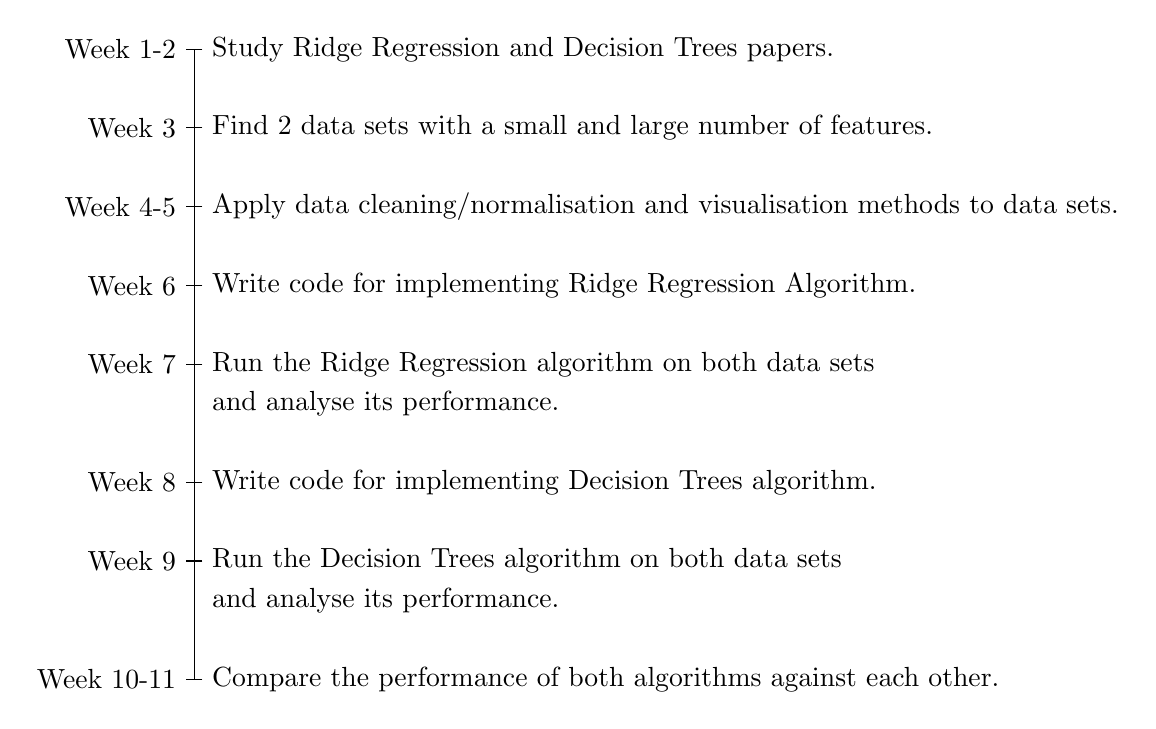
\begin{tikzpicture}
        
    \draw (0,0) -- (0,8);

    \foreach \y in {0,1.5,2.5,4,5,6,7,8}
    \draw (3pt, \y cm) -- (-3pt, \y cm);

    \draw (0,8) node[left=3pt] {Week 1-2} node[right=3pt] {Study Ridge Regression and Decision Trees papers.};
    \draw (0,7) node[left=3pt] {Week 3} node[right=3pt] {Find 2 data sets with a small and large number of features.};
    \draw (0,6) node[left=3pt] {Week 4-5} node[right=3pt] {Apply data cleaning/normalisation and visualisation methods to data sets.};
    \draw (0,5) node[left=3pt] {Week 6} node[right=3pt] {Write code for implementing Ridge Regression Algorithm.};
    \draw (0,4) node[left=3pt] {Week 7} node[right=3pt] {Run the Ridge Regression algorithm on both data sets };
    \draw (0,3.5) node[right=3pt] {and analyse its performance.};
    \draw (0,2.5) node[left=3pt] {Week 8} node[right=3pt] {Write code for implementing Decision Trees algorithm.};
    \draw (0,1.5) node[left=3pt] {Week 9} node[right=3pt] {Run the Decision Trees algorithm on both data sets};
    \draw (0,1) node[right=3pt] {and analyse its performance.};
    \draw (0,0) node[left=3pt] {Week 10-11} node[right=3pt] {Compare the performance of both algorithms against each other.};
            
\end{tikzpicture}
    
\subsection{Term 2}

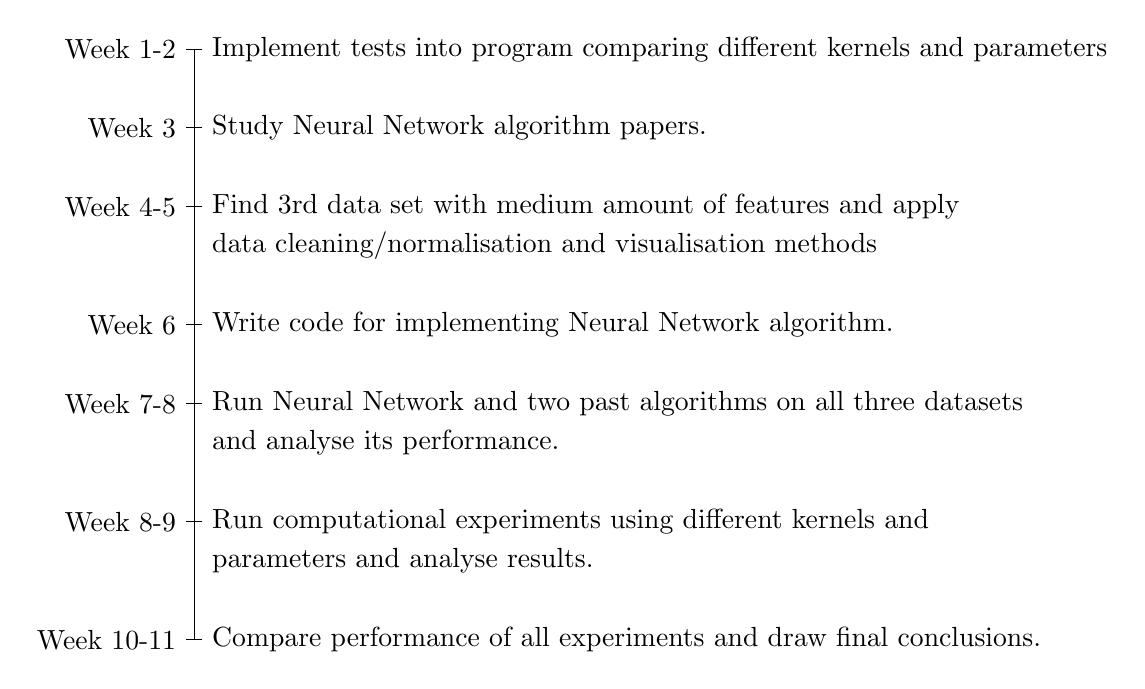
\begin{tikzpicture}
        
    \draw (0,0) -- (0,7.5);

    \foreach \y in {0,1.5,3,4,5.5,6.5,7.5}
    \draw (3pt, \y cm) -- (-3pt, \y cm);

    \draw (0,7.5) node[left=3pt] {Week 1-2} node[right=3pt] {Implement tests into program comparing different kernels and parameters};
    \draw (0,6.5) node[left=3pt] {Week 3} node[right=3pt] {Study Neural Network algorithm papers.};
    \draw (0,5.5) node[left=3pt] {Week 4-5} node[right=3pt] {Find 3rd data set with medium amount of features and apply};
    \draw (0,5) node[right=3pt] {data cleaning/normalisation and visualisation methods};
    \draw (0,4) node[left=3pt] {Week 6} node[right=3pt] {Write code for implementing Neural Network algorithm.};
    \draw (0,3) node[left=3pt] {Week 7-8} node[right=3pt] {Run Neural Network and two past algorithms on all three datasets};
    \draw (0,2.5) node[right=3pt] {and analyse its performance.};
    \draw (0,1.5) node[left=3pt] {Week 8-9} node[right=3pt] {Run computational experiments using different kernels and};
    \draw (0,1)  node[right=3pt] {parameters and analyse results.};
    \draw (0,0) node[left=3pt] {Week 10-11} node[right=3pt] {Compare performance of all experiments and draw final conclusions.};
            
\end{tikzpicture}
